\chapter{Perception of Volumetric Illustrative Effects Visualizations within OST AR} \label{Chap:PerceptionStudy}

\begin{figure}[bt]
    \centering
    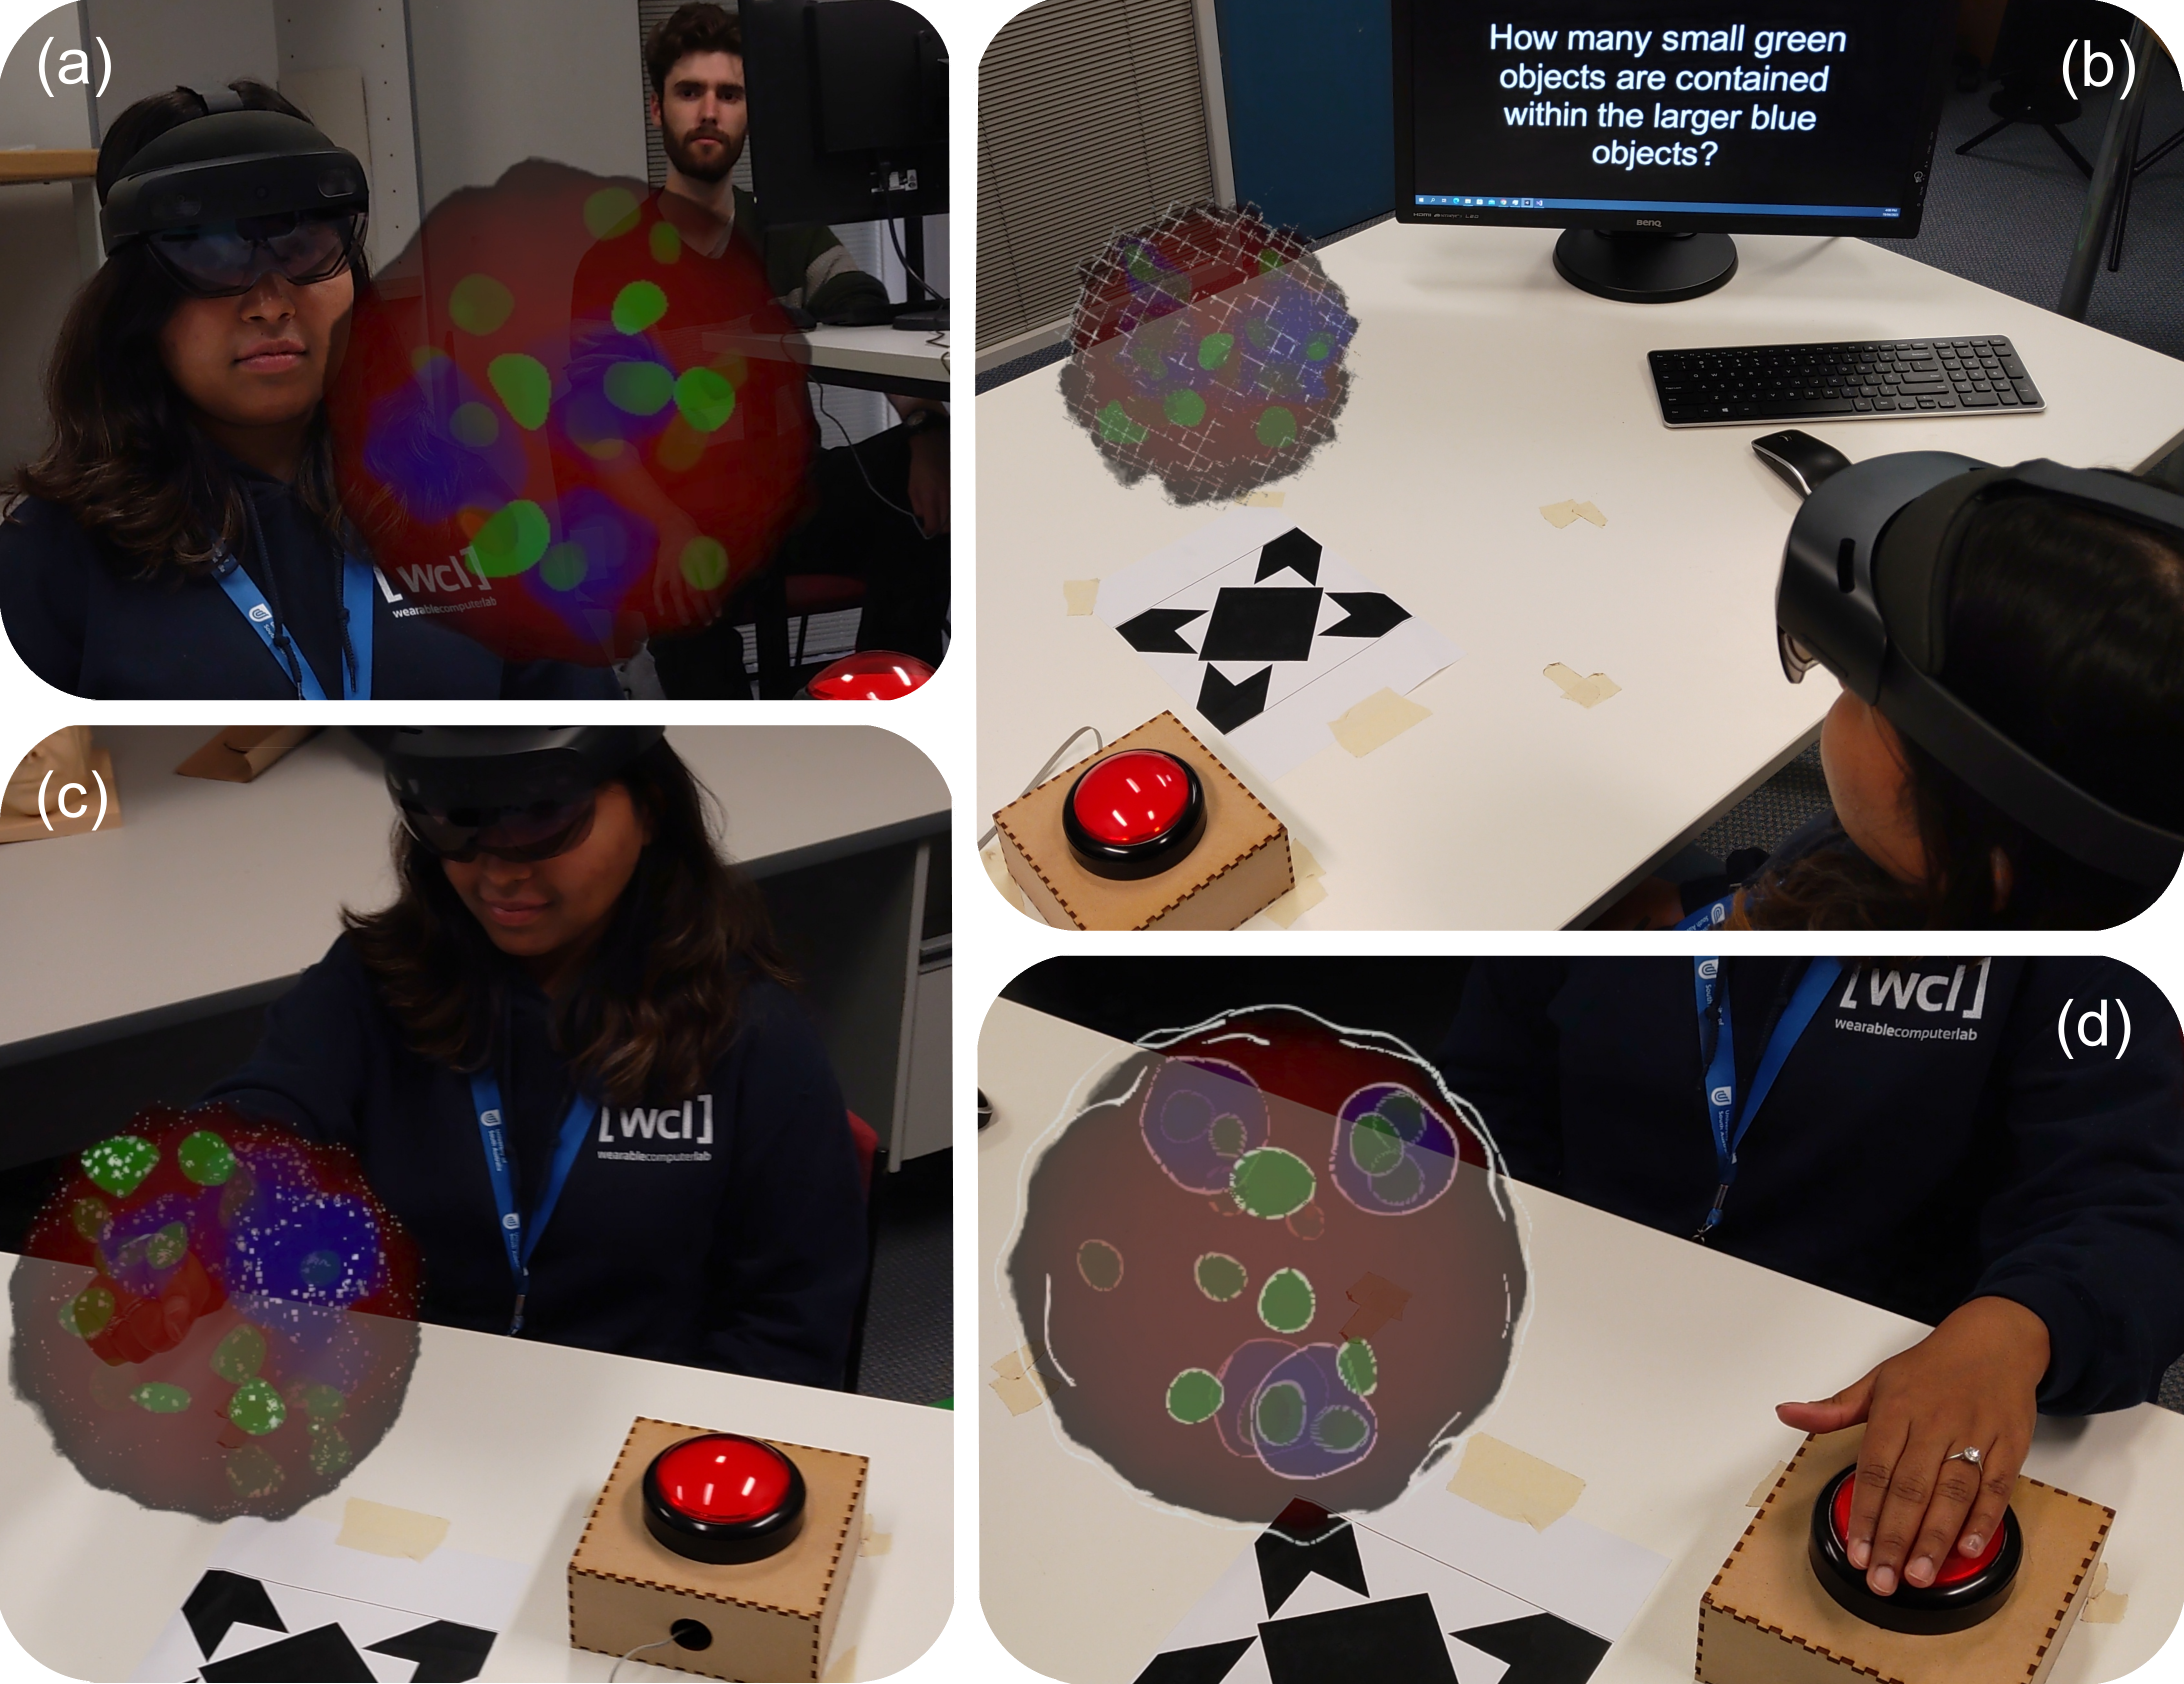
\includegraphics[width=\columnwidth]{Chapter5/Images/PerceptionStudyPhotos.png}
    \caption[This image shows the study environment in which the study was found in and all four of the conditions listed in \autoref{Chap:VolumetricX-rayVision}.]{
    These images show the study environment in which the study was found in and all four of the conditions listed in \autoref{Chap:VolumetricX-rayVision}.
    All these images were taken using an external HoloLens2's camera while observing a user interacting with the study.
    (a) Displays \textit{no \gls{virt}} and shows the participant performing the task while being observed by the researcher.
    (b) The \textit{Hatching} \gls{virt} illustrates a task perspective similar to the participants with all major interfaces visible in the photo.
    (c) An image of the participant counting the small green objects with their fingers while the visualization utilizes the \textit{stippling} \gls{virt}.
    }
    \label{fig:PerceptionStudyPhotos}
\end{figure}

% Explain this field
% Very few studies have researched how easily a person can look through \glspl{X-ray Visualization}.
% Direct Volume Rendering has several issues, one being that it is possible for viewers to miss key details within a volume. 
% This may likely be problematic on top issues like having an impaired sense of depth when previously tested in Augmented Reality~\cite{Sielhorst2006} that have been caused by \gls{dvr} objects on an \gls{ost} \gls{ar} \gls{hmd}s.

This chapter evaluates the \glspl{virt} presented in \autoref{Chap:VolumetricX-rayVision} to see if a measurable improvement can be observed when identifying individual graphical objects in a mixed reality environment.
This is critical for identifying foreign masses within the human body, allowing more rapid and accurate diagnosis and determining how compelling these visualizations would be for a given surgery. 
% Explain this study
% This chapter explores how well participants can determine what data exactly can be found in a given volume and identify individual objects when it is presented to them as a 3D volume rendering and
% \glspl{virt} are used to determine if they helped or hindered a person's ability to analyze a volume and how accurate that perception was visual.
By evaluating how participants comprehend the space and how they could categorize foreign masses, this research aims to determine if \glspl{virt} supports people's ability to understand data parameters.
%We then analyze this further by asking if users can accurately estimate the objects grouped into a smaller space.
% This provided us with some knowledge that depth perception is working better than 2cm accurately and also let us begin to understand the issues with visualizations like this.
%We were unsure if a person could clearly determine if an object was inside of another object or not. 

Illustrative rendering techniques enhance viewers' understanding of precise volume boundaries, facilitating the identification of relationships between objects. 
Practical applications of these techniques are evident in scientific illustrations, particularly in fields such as entomology and medicine~\cite{Philbrick2019, Maciejewski2008}. Artistic renderings of human anatomy have a long history, with "Gray's Anatomy"\cite{Coskun2022, Preim2005}.

% Why is this study needed
Understanding the content within a volume through an \gls{X-ray Vision} effect is important, as being able to see an object clearly is required for any visualization.
The more an effect distracts from the information it is trying to present, the less useful it becomes.
The following study aims to evaluate the effect these \gls{X-ray Visualization}s have on data, and if \glspl{virt} there are any issues that will need to be overcome to utilize any given \gls{virt} in a real-world scenario.

%
% Maybe move this stuff lower.
%

% Explaining how this fits into the study
% Findings from \autoref{Chap:X-ray Implemntion} indicated that the user's ability to look through does not seem dependant on the ability to look through the physical object, but Rather the visualization itself.
% The participants from this study seemed to struggle to focus on both the visualization and the real world simultaneously.
% This allowed us to counterbalance our study better and greatly expand the amount of data it could visualise. 

% Explain how This chapter is relevant to the rest of the thesis
%This chapter presents a study that takes the previously proposed VIRTs shown in "\autoref{Chap:X-ray Implemntion} \glspl{X-ray Visualization}" and asks participants to account for the amount of a type of artifact that appears.
%Since we didn't have to have a shape that represents the real-world body for this study, every iteration in the experiment used a unique set of shapes.

% The Road Map For the chapter.
%This chapter will elaborate on theoretical values and issues that \glspl{virt} have seen in other mediums(Mobile~\cite{Chen2012}, Desktop~\cite{Chen2012, Lawonn2013, Bruckner2007} and art~\cite{Rheingans2001, Gerl2006}) and what using these as an X-ray visualisation may cause.
%Then, 
%Details of the given user study's methodology, including the study environment, participant details, stimuli, and procedure, will be presented. 
%This will be followed by an analysis of this study's results, a detailed discussion, and lessons learned.

% Reintroducing the VIRTs in the sense of how easy they are to perceive
\section{Volumetric Illustrative Rendering Techniques}
\begin{figure}[bt]
    \centering
    
\includegraphics[width=\columnwidth]{Chapter5/Images/CountingVolumesReducedImage.png}
    \caption{The conditions that were used in this study are displayed as the volumes they are represented as.}
    \label{fig:CountingConditions}
\end{figure}

% Talk about the difficulties this chapter is aiming to fix
Artistic effects are generally chosen over utilizing transparent objects because transparent objects can be difficult to place within a virtual space.
This is because it is difficult to even in the real world to determine if a transparent object is inside or behind another object~\cite{Pisanpeeti2017}.
While realistically rendering a scene in \gls{mr} will provide you with the best possible results regarding accuracy, research has determined that better spatial understanding can be found by using a sketch or cartoon-based rendering~\cite{Wijayanto2023}.
Neither stippling nor hatching has been used much using any \gls{mr} immersive devices, but it has seen a lot of use with 3D displays~\cite{Bui2015}.

Each different \gls{virt} uses different techniques to indicate the shape and surface of the object it is trying to represent. 
\textit{Halos} work well to highlight objects and have been shown to improve depth perception~\cite{Lawonn2018, Svakhine2009, Joshi2008, Shen2014}.
Both \textit{Stippling} and \textit{Hatching} are able to illustrate the location of major surfaces in relation to each other, which should make it simpler to determine which objects are which.
Stippling accomplishes this by applying stippling to each different type of object, allowing a better sense of space~\cite{Busking2007}, while Hatching accomplishes this by changing the angles of the lines~\cite{Frech1960}.

This Chapter focuses on the \glspl{virt} revealed in \autoref{Chap:VolumetricX-rayVision}: \textit{Halo}, \textit{Hatching} and \textit{Stippling}.%\autoref{sec:X-ray vision}
The design of these \glspl{virt} is shown in \autoref{fig:CountingConditions}, utilizing the volumes that could be created by the Random Volume Generation system shown in \autoref{sec:VolumetricDataGeneration}.


\section{User Study}  \label {sec: User Studies Study 1}


%Mention similar research (1 - 2 sentences)
%Explain what the goals of this study are
% What this study aimed at achieving 
%In our first study, we want to understand whether or not a participant can understand a complete volume and identify objects within that volume. 
To access the impact that \glspl{virt} ability to identify spatial relationships between the information within the volume two tasks were designed: one of them to determine how well a user could identify objects within a volume using \gls{ost} \gls{ar}; while the other one aimed at determining how well they could identify an a grouped hierarchy.
Volumetric rendering can make spatial perception difficult due to clustering, inaccurate depth perception, and orientation~\cite{Zhou2022, Zheng2013, Bruckner2006}. 
\gls{mr} \glspl{hmd} greatly benefit these issues by enabling additional depth cues, including some stereotypical cues and motion parallax~\cite {Cutting1997, Vishton1995}. 
Still, \gls{ost} \gls{ar} \glspl{hmd} tend to have a small color or gamut and less bright and opaque colors than traditional video screens/devices~\cite{Zhan2020, Xiong2021}.


\subsection{Research Questions}
This study was designed to better understand how partial occlusion in the form of \glspl{virt} affected a user's ability to understand the data within a volume. 
Most works on the usability and perception of these effects in \gls{X-ray Vision} have either looked into where and when \gls{X-ray Vision} is needed~\cite{Wang2023, Guo2023}, what are the tolerable parameters~\cite{Santos2016}, or how to interact in a space that you cannot physically access~\cite{Blum2012, Blum2012a}.
However, there has been limited work in general on the impact of the use of \gls{mr} \glspl{hmd} when using \gls{dvr} techniques~\cite{JunYoungChoi2018, Cecotti2021, Fischer2020} with very few papers focused on \gls{ost} \gls{ar}~\cite{Sielhorst2006}. 
This has led to a great deal of potential unknowns for how \glspl{virt} being ended \gls{ost} \gls{ar} may impact how users and the limited information which existed on the impact that \glspl{virt} could have on the perception of volumes answers, the following research questions were pursued by this study where: 

\begin{enumerate}[label=RQ.\arabic*]
    \item Can \glspl{virt} aid a person’s comprehension of a volume when determining individual objects using direct volume rendering?  
    \item What is the impact of different \glspl{virt} on participants' self-reported cognitive load and usability?
    \begin{enumerate}[label=RQ.2.\arabic*]
       \item Is this effect noticeable via the differences between participant behaviour (hand, head, and eye movements) between \glspl{virt}? 
    \end{enumerate}
\end{enumerate}

\subsection{Tasks}
\begin{figure}[tb]
    \centering
    \includegraphics[width=\columnwidth]{Chapter5/Images/TaskDescription.png}
    \caption[A visual description of how the task users in this study were asked to conduct using a volume with 22 green artifacts.]{A visual description of how the task users in this study were asked to conduct using a volume with 22 green artifacts. On the left-hand side, users were asked to count all of the green artifacts, while on the left-hand side, they were asked to count all of the objects nested inside of the blue artifacts. All of the green cells that participants were asked to count for each task are marked with a white outline and counted with a number to the top right of each green artifact.}
    \label{fig:TaskDescription}
\end{figure}

% What inspired this study design and where can similar ones be found
The study design was based on work done in the field of visual analytics and was influenced by studies within the field of volume rendering and visual analytics~\cite{Laha2012, Laha2014, Laha2013}. 
To understand what the participants could comprehend about the volumes with a range of given \glspl{virt}. 
Investigating how well participants could record information within the volume using \glspl{virt}.
This was compiled by generating a set of 7680 volumes that all utilized the same range of data, allowing a unique volume that conformed to a set of predefined rules and had users report on the frequency of artifacts in the object.

\subsubsection{Count All}
In the first task, participants were asked to summarize a visual data set (shown in \autoref{fig:DifferentAmounts}) by asking them to "Count all of the small green objects throughout the entire volume".
This is called the "\textit{Count All}" task for simplicity.
The desired behaviour participant is illustrated on the left-hand side of \autoref{fig:TaskDescription}. 
This task was proposed in relation to \gls{dvr} usability by Laha et al.~\cite{Laha2016}, and a variation of it was used by Munzener et al.~\cite{Munzner2014}.
The aim of the question was to determine how easily people can identify individual objects within the volume and the effect of \glspl{virt} on their accuracy.

\subsubsection{Count Nested}
In the second task, participants were asked to count the "small green objects located within the larger blue objects." 
This was called the "\textit{Count Nested}" task. 
The desired behaviour participant is illustrated on the right-hand side of \autoref{fig:TaskDescription}. 
This task was intended to determine how accurately people understand the spatial relationships within a volume and the effect of \glspl{virt} on their accuracy. Specifically, the goal of this research was to understand if \glspl{virt} assists people in identifying if an object is in front of, inside, or behind another object. 


\subsection{Hypotheses} \label {sec: User Studies Hypothesis}
\begin{enumerate}[label=H.\arabic*, series=Hypotheses] 

    \item Participants will identify all of the objects more accurately using the \textit{halo} \gls{virt} in the \textit{Count All} task (R1);
    \textit{Piringer et al.~\cite{Piringer2004} have shown that the halo effect can allow for people to rapidly find objects within large 3D datasets and DVR visualizations}
    
    \item Participants will identify all of the objects faster using the \textit{halo} \gls{virt} in the \textit{Count All} task (R1).
    \textit{The same studies as above have shown that \textit{halo} can improve identification time ~\cite{Piringer2004}};
    
    \item Participants will identify all of the objects more accurately using the \textit{hatching} \gls{virt} in the \textit{Count Nested} task (R.1).
    \textit{These visualizations have been designed to enable better depth perception for users and should be able to aid participants when counting large amounts of objects};
    
    \item Participants will identify all of the objects fastest when either using the \textit{hatching} or \textit{stippling} \glspl{virt} in the \textit{Count Nested} task (R.1).
    \textit{As in the previous study in this dissertation and in other similar studies, the visualizations should enable a more accurate view of the dataset. This effect can be seen without volume rendering in works that don't use volume rendering, and I believe that this will carry over into this experiment~\cite{Martin-Gomez2021}};

    \item Participants will move their hands, eyes, and heads at a lower rate when they are using the \textit{halo} \gls{virt} (R.2.1).
    \textit{The embodied cognition field looks at instances when the body plays a significant causal role in a person's cognitive processing~\cite{Raab2019, Wilson2013}. I expect that people would move their heads and eyes more rapidly when trying to solve a difficult problem~\cite{Wilson2013}. This is likely to take the place of hand motions to help them count, like using their fingers to count and pointing at the objects~\cite{Wilson2013}, but could also be seen in with rapid eye movements};
    
    \item The \textit{halo} \gls{virt} will be the most preferable and least cognitively demanding for identification tasks (R2);
    \textit{When other studies have utilized similar methods, they have found that a silhouette or outline has been more appealing to participants~\cite{Martin-Gomez2019, Fischer2020a}};
    
\end{enumerate}

\subsection{Participants} \label {sec: User Study Perception Participants}
24 participants were recruited for this study from a pool of students, faculty and staff from the University of South Australia aged between 21 and 37 years old ($mean = 26.95, \sigma = 4.47$), 6 female, 18 male, with little(9) to no (15) experience with medical data.
Their experience using MR systems varied, with 8 people using them daily, 5 using them weekly, 6 using them monthly, 2 using them rarely, and 3 using them for the first time.
All participants were asked to declare if they had any major vision impairments that could not be corrected during the recruitment process. If this was the case, they would have been asked not to participate in the study. 

\subsection{Procedure}  \label {sec: User Studies Study 1 Design}
 %PreAt the start of starting the study, participants were required to read and fill out an information sheet, content form, and demographic survey. 
Participants were asked to sit down and complete eight training exercises to familiarise them with the task of each condition containing either 13 or 14 objects to count in total.
No data was recorded during this phase, and the participants were encouraged to talk to the examiner. 
After this, participants were allowed to take a break before starting the study.

\subsubsection{Task} \label{sec:PerceptionTaskDesgin}

\begin{figure}[bt]
    \centering
    
\includegraphics[width = \columnwidth]{Chapter5/Images/DifferentAmountsOfVIRTs.png}
    \caption{5 volumes each using \textit{no \gls{virt}} each with a different number of green objects to count.}
    \label{fig:DifferentAmounts}
\end{figure}

% the task users were asked to perform
Each participant was asked to \textit{count all} of the small green objects throughout the scene (\textit{Count All}) or only the green objects located within one of the blue regions (\textit{Count Nested}).
%To not confuse the participants, we would have them answer each question in a group of 15 and display the question on a monitor for them to remind them each time.
To ensure clarity, participants would be tasked with answering the same question for each \gls{virt} at the same time before moving forward to the other question for that same \gls{virt}. 
This group of 15 would consist of 3 repetitions of 5 conditions shown in \autoref{fig:DifferentAmounts}, each containing 14, 16, 18, 20, and 22 objects to count.
The order in which the \glspl{virt} was presented was completely counterbalanced.

This was done to ensure the participants were aware of which task they were being asked to perform.
Every time the question changed, the examiner would verbally inform the participant. 
The order in which these questions were asked throughout the study would be shuffled to remove possible learning effects. 
The question would also be displayed on the nearby computer screen if the participant was confused, and this would be changed for a prompt telling the participant the question would change each time.
This allowed us to test how well participants could identify objects within the scene and the spatial location and hierarchy of the objects within the scene.

% Data collection
Participants were given a large red button (called the task button) that allowed them to start each iteration presenting the visualization.
Participants were required to press the task button before giving their answer.
Participants would then be prompted by a computer monitor where they would input their answer via a keyboard.
During the times between the task buttons being pressed, the time is taken to start, and it would finish when they pressed it again to signal the end of the condition. 
When Participants are prompted to provide their answer via the nearby keyboard and monitor. 
When Participants pressed the task button again, the next iteration of the study would begin. 
their hand, head, and gaze movements were tracked. 
%Their voice was also recorded - Extend on this tom, and the examiner would take notes regarding any unusual behaviour they presented, such as counting with their hands or voice.

%Questionnaires and Post-Study
Between each condition, participants were asked to take a questionnaire that consisted of a PAAS~\cite{Paas2003}, a SUS~\cite{Lewis2018}, and a question promoting them to quantify between 0(worst) and 5(best) how well they could observe all the objects in the volume as well as giving them the option to tell us what they liked and disliked about the \gls{virt} which is reported in \Cref{app:Chapter5Comments}.
The post-study questionnaire asked the participants to rank how they believed they performed with all of the \glspl{virt}, and how easy they were to use, and they were given the opportunity to explain their answers (reported in \Cref{app:Chapter5Comments}). These answers were then used to confirm a correlation between how the participants answered each condition.

\begin{figure}
    \centering
    \includegraphics[width=\columnwidth]{Chapter5/Images/SketchOfStudy2TableLayoutPerception.png}
    \caption[The layout of the study area (the participants desk space) the participants had around them for the perception experiment.]{The layout of the study area (the participants desk space) the participants had around them for the perception experiment. Distances are in center meters}
    \label{fig:PerceptionStudySpace}
\end{figure}

\subsubsection{Pilot Study}
%Study Settings and Parameters
The amount of objects in this study was decided by comparing this study research to similar studies in graph visualizations that would use up to 20 nodes in their visualizations~\cite{Yoghourdjian2018}. 
A separate pilot study was conducted using 5 participants (1 female 4 male) who were aged between 21 - 57 years old. 
This study used a similar procedure to the one listed in \autoref{sec:PerceptionTaskDesgin}, which used a wider range of values from 9 green objects to 27.
Only the \textit{no \gls{virt}} condition was used in the pilot study.

The results from this study showed that they struggled to count past 18 when presented with the baseline condition.
All visualizations were randomly generated for each study iteration, following a predefined set of rules laid out in the previous chapter (\autoref{Chap:VolumetricX-rayVision}).
This caused the decision to have numbers ranging around 18 objects the participants needed to count. 
%Allowing for some conditions that we were confident participants could perform well and others they would have likely struggled with when using the \textit{no \gls{virt}} condition. 

\subsection{Study Environment}

The study took place in a dimly lit room with multiple light sources (windows and stage lighting) and utilized the space shown at the centre of the room shown and detailed in \autoref{fig:PerceptionStudySpace}.
The visualization would appear 15cm above the visualization marker.
Participants could move the computer screen, keyboard, and button to a preferred location, but each user studied started in the same position.
Participants were seated at a desk in the center of the room and observed throughout the study by a researcher as shown in \autoref{fig:PerceptionStudyPhotos} a). The study was facilitated and built upon using the Unity Engine\footnote{\url{https://unity.com/releases/editor/whats-new/2019.4.3}}, with the Microsoft Hololens 2\footnote{\url{https://www.microsoft.com/en-us/hololens/}}  (\autoref{fig:PerceptionStudyPhotos}(b)) as the display modality via a wired connection utilizing the Holographic Remoting Player\footnote{\url{https://learn.microsoft.com/en-us/windows/mixed-reality/develop/native/holographic-remoting-player}} to a desktop PC. The desktop PC featured an Intel i5 with an Nvidia Geforce GTX 2070 GPU, running at between 60-90 FPS during the study. 
Participants would either be given a task button on either their left or right side for this study.

\section{Results} \label{sec:sdfResultsPerception}
This section contains the analysis of the data collected in both studies.
All values with a p-value $<$ 0.1 have been reported, while only p-values $<$ 0.05 are considered significant.


\begin{figure}[bt]
    \centering
    \includegraphics[width=\columnwidth]{Chapter5/Images/CountingEverythingMainResults.pdf}
    \caption[The accuracy, or difference between the participant's and real answers, when counting all green objects within the volume by the \glspl{virt} and the number of objects they were asked to count.]{The accuracy, or difference between the participant's and real answers, when counting all green objects within the volume by the \glspl{virt} and the number of objects they were asked to count.
    Confidence intervals (CL = 95\%) calculated from the post-hoc emmeans between all conditions are shown as boxes on each error bar.
    Significance bars have been omitted as all conditions are significant}
    \label{fig:CountingEveryThingMainResultsAllShownLineGraph}
\end{figure}


%We were most interested in for the object identification study.
In this study, while the participant was observing the volume, the system tracked: 
\begin{itemize}
    \item The participants' accuracy. The absolute difference between the amount of green objects the participants counted($p$) and the actual amount of objects there was($a$);
    \item The time required for a participant to count the number of green objects.
    \item and user behaviour details were recorded this included information required to track:
        \begin{itemize}
            \item Eye Movements
            \item Head Movements
            \item Hand Movements
        \end{itemize}
\end{itemize} 
For the analysis of errors and time, linear mixed models were conducted. This approach accounts for individual differences between participants in repeated measures and allows us to also examine the effect of the number of objects.~\cite{Kaptein2016, Adams2022}.
% A mixed linear model examined the differences across all variables measured for \autoref{sec:sdfResultsPerceptionAccuracy} and \autoref{sec:sdfResultsPerceptionTimeRequired}. 
% This model accounted for the individual differences between the participants and allowed us to permit model specification-based interaction effects if possible, allowing us to look into the effect the number of objects may have on the VIRTs.
%Allowing us to look into the number of objects' effect on the VIRTs.
Both models were specified with the fixed factors of the \glspl{virt} designed in \autoref{Chap:VolumetricX-rayVision}, the number of objects the user was required to count, and the interaction effect between them plus a random effect of the participant on the intercept. Significance values were extracted using Type II Wald chi-square tests, and where appropriate, pairwise post hoc comparisons were conducted using Tukey’s \gls{hsd} for multiple comparisons.
%Results for the two questions asked
%"How many smaller green blobs are there?"

\subsection{Accuracy (H.1 \& H.3)} \label{sec:sdfResultsPerceptionAccuracy}

% (Moved this from above as it only applies to this subsubsection
The accuracy of the participant responses was measured as the difference between the correct answer and the answer given by the participant. The model for accuracy in the \textit{Count All} task showed a significant fixed effect between the \glspl{virt} ($\chi$2(3, N = 24) = 777.083, p $<$ 0.0001), and the number of objects also showed a significant fixed effect ($\chi$2(4, N = 24) = 146.190, p $<$ 0.0001), with a significant interaction effect (($\chi$2(3, N = 24) = 34.605, p $<$ 0.0001)). 
These results are illustrated in \autoref{fig:CountingEveryThingMainResultsAllShownLineGraph}.

The post hoc pairwise comparisons between the \glspl{virt} showed significant differences for all combinations (p $<$ 0.0001). 
\textit{Halo} had the highest accuracy, followed by \textit{no \gls{virt}}, \textit{stippling}, and \textit{hatching} in descending order.
Comparison between the different numbers of objects showed significant differences between 14 and 22, 16 and 24, 16 and 22, and 18 and 24 objects (p $<$ 0.0001), 14 and 28 (P = 0.0005), 16 and 18 objects (p = 0.0247), and 23 and 25 objects (p = 0.0033). The accuracy was lower when the participant had more objects to count in all of these pairs.
% These results showed that the more objects that existed, the less accurate the users tended to be.

The Post hoc Pairwise comparison for the interaction between the conditions had 138 significant effects with a p-value $<$ 0.05. 
To summarize these effects, most visualizations showed a significant difference in themselves when the difference between the number of objects the participant had to count was greater than 4, regardless of \glspl{virt}.
The one exception to this rule was the \textit{halo} visualization, which showed no significant differences against itself when the participant was required to count any number of objects.
A full breakdown of the results can be found in \Cref{apendix:ErrorWhenCountingEverything}.


%For clarity noticable trends noticed in \Cref{apendix:ErrorWhenCountingEverything}
For conditions with fewer objects to count, \textit{hatching} was unlikely to be significant when compared to conditions using \textit{stippling} with more objects to count. 
There was a high level of significance for the inverse, though (when there were fewer objects to count using \textit{stippling} than \textit{hatching}).
Generally, \textit{hatching} and \textit{stippling} showed a very significant difference when compared to \textit{no VIRT} and \textit{halo}. 
All other interaction pairs not previously mentioned showed a significant difference from one another. A full table of these effects can be found in the supplemental materials.

For the \textit{Count Nested} task, the model showed a significant fixed effect between the \glspl{virt} ($\chi$2(3, N= 24) = 347.053, p $<$ 0.0001). No significant effect of the number of objects or significant interaction effect was shown. 
The post hoc pairwise comparison of \glspl{virt} showed significant results between \textit{halo} and \textit{hatching}, \textit{halo} and \textit{stippling}, \textit{hatching} and \textit{no \gls{virt}}, \textit{hatching} and \textit{stippling}, \textit{no \gls{virt}} and \textit{stippling} (p $<$ 0.0001), and \textit{halo} and \textit{no \gls{virt}} (p = 0.0001). 
%The results were similar to when all green objects were counted.
\textit{Halo} had the highest accuracy, followed by \textit{no \gls{virt}}, \textit{stippling}, and \textit{hatching} in descending order. 
%This likely indicates that participants had no real issue determining what was inside the blue objects. Instead, the \glspl{virt} themselves appear to have a bigger impact on the ability to count the objects accurately.
%However in this case, as can be seen in \autoref{fig:CountingWithinTheBlueMainResults}, it was uncommon for participants to get any errors when using the \textit{halo} \gls{virt}. 


\begin{figure}[tb]
    \centering
    \includegraphics[width=\columnwidth]{Chapter5/Images/CountingNestedMainResults.pdf}
    \caption{The accuracy of participant responses when completing the \textit{Count Nested} task.
    The error bars indicate each \gls{X-ray Visualization}'s confidence levels (CL = 95\%).
    Significance bars have been omitted as all conditions are significant}
    \label{fig:CountingWithinTheBlueMainResults}
\end{figure}

\subsection{Time Required (H.2 \& H.4)} \label{sec:sdfResultsPerceptionTimeRequired}
% The time it took to answer these questions.
The model for the time spent on the \textit{Count All} task showed a significant effect between the number of objects viewed ($\chi$2(4, N= 24) = 85.9544, p $<$ 0.0001). There was no significant fixed effect between the four conditions and no significant interaction effect. 
% To further evaluate these findings, post hoc pairwise comparisons using Tukey’s HSD for multiple comparisons. 
The post hoc pairwise comparison of the different numbers of objects showed significant differences between 14 and 22, 16 and 22 (p $<$ 0.0001), 14 and 20 (p = 0.0008), and 18 and 22 (p = 0.0055). 
%These results show that the more objects

\begin{figure}[bt]
    \centering
    %\includegraphics[width=\columnwidth]{Chapter5/Images/CountingOnlyWithinTheBlueTimeTaken.pdf}
    \includegraphics[width=\columnwidth]{Chapter5/Images/CountingTimeRequired.pdf}
    \caption[The time required to complete each interaction of a task for each \gls{virt} for both the \textit{Counting Everything} and \textit{Counting Nested} tasks.]{The time required to complete each interaction of a task for each \gls{virt} for both the \textit{Counting Everything} and \textit{Counting Nested} tasks.
    The error bars indicate each \gls{X-ray Visualization}'s confidence levels (CL = 95\%).
    Significance differences are displayed as the lines on the right side of the graph stars indicate significance (* = p $<$ 0.05; ** = p $<$ 0.01; *** = p $<$ 0.001).
    }
    \label{fig:CountingOnlyWithinTheBlueTimeTaken}
\end{figure} the participants had to count, the longer it took them to complete the task, particularly when the count differed by four objects.

The model for the time spent on the \textit{Count Nested} task showed a significant fixed effect between the four \glspl{virt} ($\chi$2(3, N= 24) = 85.9544, p $<$ 0.0001). In contrast to counting all objects, the fixed effect number of objects shown only showed some variability ($\chi$2(4, N= 24) = 8.5963, p $=$ 0.07202), and no significant interaction effects were found. 
The post hoc comparison between the \glspl{virt} showed significant differences between \textit{halo} and \textit{hatching}, \textit{halo} and \textit{stippling}, \textit{hatching} and \textit{no \gls{virt}} (p $<$ 0.0001), \textit{hatching} and \textit{stippling} (p = 0.0010), and \textit{no \gls{virt}} and \textit{stippling} (p = 0.0143). 
%\autoref{fig:CountingOnlyWithinTheBlueTimeTaken} shows \textit{halo} was the fastest condition for participants, closely followed by \textit{no \gls{virt}}, with \textit{stippling} and \textit{hatching} being significantly slower than both. 

A Kendall correlation test was used to determine if the time spent by each participant correlated to their accuracy. 
When only counting the green objects contained within the larger blue objects, a significant relationship between the time required and range of error was found with a low to moderate amount of correlation $\tau = -0.18$ (z = -9.3074, p $<$ 0.0001), showing that participants tended to do better when they took more time some of the time. 
When counting all of the objects, almost no relationship was found between the time required and accuracy $\tau = -0.03831766$ (z = -1.8507, p = 0.06422), suggesting that taking more time when performing this task did not help improve accuracy. 

%(Optional) present analysis for voice and gesturing analysis. 
\subsection{User Behavioural Analysis (H.5)} \label{sec:PerceptionBehavioralResults}
This section focuses on how the participants' behaviour reacted to the four conditions. 
Over the course of the overall distance, participants would have moved their heads, gaze, and hands where tracked. 
This is then divided by the time each condition took to allow us to view the average speed at which participants moved.
The headset's and hand's distance was tracked by calculating the amount its position had moved relative to the visualisation between every 16ms and summing these results.
When the hands were not in front of the user, their distance was not tracked.
Eye Gaze's distance was measured by tracking the distance a user's eye gaze would move within a 2m radius from the participant's current position in each frame minus the same distance that the head gaze would have provided. 

\begin{figure}[tb]
    \centering
    \includegraphics[width=\columnwidth]{Chapter5/Images/CountingHeadVel.pdf}
    \caption[Box plots showing how much each participant moved their head to view the volume between the different \gls{virt} conditions for both the \textit{Counting Everything} and \textit{Counting Nested} tasks.]{Box plots showing how much each participant moved their head to view the volume between the different \gls{virt} conditions for both the \textit{Counting Everything} and \textit{Counting Nested} tasks.
    The error bars indicate each \gls{X-ray Visualization}'s confidence levels (CL = 95\%).
    Significance differences are displayed as the lines on the right side of the graph stars indicate significance (* = p $<$ 0.05; ** = p $<$ 0.01; *** = p $<$ 0.001).
    }
    \label{fig:HeadsetMovementPerception}
\end{figure}

% The model for the users head motion when counting nested
The model for the participants' head motion velocity for the \textit{Counting Nested} task showed a significant fixed effect between the various \glspl{virt} ($\chi$2(3, N= 24) = 54.9095, p $<$ 0.0001). 
The fixed effect number of objects and interaction effects both found no significant effects. 
The post hoc comparison between the \glspl{virt} showed significant differences between \textit{hatching} and \textit{no \gls{virt}} (p $<$ 0.0001), \textit{no \gls{virt}} and \textit{Stippling} (p = 0.0001), \textit{Halo} and \textit{no \gls{virt}} (p = 0.0047), \textit{Halo} and \textit{hatching} (p = 0.0005), \textit{Halo} and \textit{no \gls{virt}} (p = 0.0049), \textit{Hatching} and \textit{Stippling} (p = 0.0205).
\autoref{fig:HeadsetMovementPerception}'s Counting Nested objects graph shows that having no \gls{virt} leads to an unpredictable reaction from the user behaviour while adding a \gls{virt} tends to restrict this.

% Results for distance head moved for motition velocity
The model for the participants' head motion velocity for the \textit{Counting Everything} task showed a significant fixed effect between the various volumetric Illustrative Renderings ($\chi$2(3, N= 24) = 32.2482, p $<$ 0.0001). In contrast to counting all objects, the fixed effect number of objects and interaction effects were found to have no significant effects. 
The post hoc comparison between the \glspl{virt} showed significant differences between \textit{halo} and \textit{stippling}, and \textit{hatching} and \textit{stippling} (p $<$ 0.0001), \textit{no \gls{virt}} and \textit{Hatching} (p = 0.0042), \textit{Halo} and \textit{no \gls{virt}} (p = 0.0047).
\autoref{fig:HeadsetMovementPerception}'s Counting Everything graph shows that the \textit{Hatching} and \textit{Stippling} \glspl{virt} required participants to move more than other \gls{virt} such as \textit{halo} or \textit{no \gls{virt}}.

\begin{figure}
    \centering
    \includegraphics[width=\columnwidth]{Chapter5/Images/CountingHandVel.pdf}
    \caption[A graph showing the speed at which participants moved their hands in this experiment when the different \glspl{virt} were being utilized for both the \textit{Counting Everything} and \textit{Counting Nested} tasks.]{A graph showing the speed at which participants moved their hands in this experiment when the different \glspl{virt} were being utilized for both the \textit{Counting Everything} and \textit{Counting Nested} tasks.
    The error bars indicate each \gls{X-ray Visualization}'s confidence levels (CL = 95\%).
    Significance differences are displayed as the lines on the right side of the graph stars indicate significance (* = p $<$ 0.05; ** = p $<$ 0.01; *** = p $<$ 0.001).
    }
    \label{fig:PerceptionSpeedHandsMoved}
\end{figure}

% Results for Hand Motion
The model for the participants' head motion velocity for the \textit{Counting Everything} task showed no significant results. 
However, The model for the \textit{Counting Nested} task showed a significant fixed effect between the \glspl{virt} ($\chi$2(3, N= 24) = 11.7432, p $=$ 0.0083), but both the fixed effect for the different amounts of countable objects and the interaction effect showed no significant results.
The post hoc comparison between the various \glspl{virt} showed that when participants were using the \textit{Halo} \gls{virt}. 
\autoref{fig:PerceptionSpeedHandsMoved}, they would move their hands significantly faster than they would during the \textit{Stippling} task (p = 0.0057).

\begin{figure}
    \centering
    \includegraphics[width=\columnwidth]{Chapter5/Images/CountingEyeVel.pdf}
    \caption[Box plots relating to the speed at which participants moved over different eye gazes.]{Box plots relating to the speed at which participants moved over different eye gazes.
    The error bars indicate each \gls{X-ray Visualization}'s confidence levels (CL = 95\%).
    Significance differences are displayed as the lines on the right side of the graph stars indicate significance (* = p $<$ 0.05; ** = p $<$ 0.01; *** = p $<$ 0.001).
    }
    \label{fig:PerceptionEyeGaze}
\end{figure}

% Results for Eye gaze for counting everything
The model for the velocity of the participants' eye gaze for \textit{Counting Everything} task showed a significant fixed effect between the different \glspl{virt} ($\chi$2(3, N= 24) = 19.347, p $=$ 0.0002) and the number of objects in total ($\chi$2(4, N= 24) = 30.759, p $<$ 0.0001). No significant interaction effect was found.
The post-hoc comparison between the \glspl{virt} showed that participants significantly moved their eyes more when using stippling compared to \textit{Halo} (p = 0.0007) and \textit{Hatching} (p = 0.0010). Some variation was also found between \textit{No \gls{virt}} and \textit{Stippling} (p = 0.0918). 
Whereas the posthoc comparison for the number of objects \textit{14} countable objects showed participants moved their eyes significantly less compared to \textit{18} (p = 0.0013), \textit{20} (p = 0.0153) and \textit{22} (p = 0.0013). The same phenomenon was found with \textit{16} countable objects as participants moved their eyes significantly fewer results against \textit{20} (p = 0.0177) and \textit{22} (p = 0.0024).

% Results for eye gaze when counting nested objects
The model for the velocity of the participants' eye gaze for \textit{Counting Nested} task showed a significant fixed effect between the different \glspl{virt} ($\chi$2(3, N= 24) = 28.1722, p $<$ 0.0001) and no significant fixed effect was found with the number of objects to count and the interaction effect.
The post-hoc comparison between the \glspl{virt} (shown in right hand side of \autoref{fig:PerceptionEyeGazeAmountOfObjectsToCount}) showed that \textit{Stippling} was significantly faster compared to \textit{Halo} (p = 0.0004) and \textit{no \gls{virt}} (p $<$ 0.0001). Participants moved significantly slower when using \textit{Hatching} when compared to \textit{no \gls{virt}} (p = 0.0108). Some variation could also be seen between \textit{Hatching} and \textit{Halo} (p = 0.0602). 

\begin{figure}[tb]
    \centering
    %\includegraphics[width=\columnwidth]{Chapter5/Images/PerceptionEyeGaze.pdf}
    \includegraphics[width=\columnwidth]{Chapter5/Images/EyeGazeAmountOfObjectsToCount.pdf}
    \caption[A plot showing the difference in velocity between the user's eye movements when different amounts of objects existed for them to see when counting everything.]{A plot showing the difference in velocity between the user's eye movements when different amounts of objects existed for them to see when counting everything.
    The error bars indicate each \gls{X-ray Visualization}'s confidence levels (CL = 95\%).
    Significance differences are displayed as the lines on the right side of the graph stars indicate significance (* = p $<$ 0.05; ** = p $<$ 0.01; *** = p $<$ 0.001).
    }
    \label{fig:PerceptionEyeGazeAmountOfObjectsToCount}
\end{figure}

\subsubsection{Subjective Results (H.6)} \label{sec:PercptionSubjectiveResults}
% What is the content in this section
This section focuses on how the participants themselves perceive the various \glspl{virt}.
By asking participants to complete the PAAS Cognitive load scale and a System Usability Scale (SUS) questionnaire. 
Paired with the asking participants "\textit{How easy was it to look at objects inside of other objects using this visualization?}".
It was possible to gain further insights into the participants' actions and behaviours. 


The results from the PAAS questionnaire for the counting only within the blue showed a significant difference between different illustrative visualizations using a Friedman rank sum test ($\chi2(3, N= 24)= 46.493, p < 0.0001$).
Post-hoc analysis with pairwise Wilcoxon signed-rank tests was conducted with a Bonferroni correction applied, comparisons showed significantly increased cognitive load between \textit{hatching} and \textit{halo} (p $<$ 0.0001), \textit{no \gls{virt}}, and \textit{halo} (p = 0.0008), \textit{stippling} and \textit{hatching} (p = 0.0003), \textit{no \gls{virt}} and \textit{hatching} (p = 0.0031). 
The PAAS questionnaire for the counting everything question showed a significant difference between different illustrative visualizations using a Friedman rank sum test ($\chi$2(3, N= 24)= 43.674, p $<$ 0.0001).
Post-hoc analysis with pairwise Wilcoxon signed-rank tests was conducted with a Bonferroni correction applied, comparisons showed significantly increased cognitive load between \textit{Hatching} and \textit{Halo} (p $<$ 0.0001), \textit{no \gls{virt}} and \textit{Halo} (p = 0.0008), \textit{Stippling} and \textit{Hatching} (p = 0.0041), \textit{no \gls{virt}} and \textit{Hatching} (p = 0.03618), and \textit{Hatching} and \textit{no \gls{virt}} (p = 0.0064).
All of the PAAS results found, shown in \autoref{fig:CountingPAASResults}, indicate that participants feel that the \textit{halo} \gls{virt} required the least cognitive load, while the \textit{hatching} and \textit{no \gls{virt}} \glspl{virt} were felt to require a much greater cognitive load.

All the PASS results for both were highly correlated $\tau = 0.77$ (z = 9.9632, p $<$ 0.001) to each other. showing that regardless of the task the participants were presented with, they felt these visualizations took a similar cognitive load.
% PASS - Separated between conditions
The correlation between the PAAS Questionnaire Results and how well participants believed they did on each condition. A significant negative relationship between them $\tau = -0.49$ (z = -6.4262, p $<$ 0.001). Showing participants' feelings at the end of the study and showcasing an accurate representation of how they viewed their performance.

\begin{figure}[bt]
    \centering
    \includegraphics[width=\columnwidth]{Chapter5/Images/CountingPAAS.pdf}
    \caption[Outcomes from the PAAS questionnaire in the counting study. Lower results indicate lower cognitive load and higher results indicate higher cognitive load.]{Outcomes from the PAAS questionnaire in the counting study. Lower results indicate lower cognitive load and higher results indicate higher cognitive load.
    Significance differences are displayed as the lines on the right side of the graph stars indicate significance (* = p $<$ 0.05; ** = p $<$ 0.01; *** = p $<$ 0.001).
    }
    \label{fig:CountingPAASResults}
\end{figure}
    
% SUS - Separated between conditions
The results from the SUS questionnaire showed a significant difference between different \gls{virt} using a Friedman rank sum test ($\chi2(3, N= 24)= 54.728, p < 0.0001$)
Post-hoc analysis with pairwise Wilcoxon signed-rank tests was conducted with a Bonferroni correction applied, comparisons showed significantly increased cognitive load between \textit{hatching} and \textit{halo} (p $<$ 0.0001), \textit{no \gls{virt}} and \textit{halo} (p $<$ 0.0089), \textit{stippling} and \textit{halo} (p = 0.015) \textit{stippling} and \textit{hatching} (p = 0.0019), and \textit{no \gls{virt}} and \textit{hatching} (p = 0.0022) (see \autoref{fig:CountingSUSResults}).
    
% Correlation between PAAS and SUS to the final questionnaire
The correlation between the SUS Questionnaire Results and how easily participants found the visualizations to use was tested where there was a significant relationship between them $\tau = 0.48$ (z = 6.2974, p $<$ 0.0001). Showing a mildly strong positive correlation between participants' feelings about their ability to use the \glspl{virt} for this task.

\begin{figure}[!b]
    \centering
    \includegraphics[width=\columnwidth]{Chapter5/Images/CountingSUS.pdf}
    \caption[Results of the SUS questionnaire for the counting study.]{Results of the SUS questionnaire for the counting study.
    Significance differences are displayed as the lines on the right side of the graph stars indicate significance (* = p $<$ 0.05; ** = p $<$ 0.01; *** = p $<$ 0.001).
    }
    \label{fig:CountingSUSResults}
\end{figure}

Responses for the question "\textit{How easy was it to look at objects inside of other objects using this visualization?}" were analyzed using a Friedman rank sum test and showed a significant difference between the various \gls{virt} ($\chi$2(3, N= 24)= 49.392, p $<$ 0.0001). 
Post-hoc analysis with pairwise Wilcoxon signed-rank tests was conducted with a Bonferroni correction applied. Comparisons showed participants found it significantly more challenging to see through the \textit{hatching} and \textit{halo}, \textit{no \gls{virt}} and \textit{halo} (p $<$ 0.0001), \textit{stippling} and \textit{halo} (p = 0.0012), \textit{stippling} and \textit{hatching} (p = 0.0005), and \textit{no \gls{virt}} and \textit{hatching} (p = 0.0030) \glspl{virt} (see \autoref{fig:CountingSeeThroughResults}).

%(Optional) Correlation between the voices and gestures and PAAS questionnaire

\section{Discussion} \label{sec:Disscussion}

\begin{figure}[!tb]
    \centering
    \includegraphics[width=\columnwidth]{Chapter5/Images/CountingEase.pdf}
    \caption{Results for the question \textit{"How easy was it to look at objects inside of other objects using this visualization?"}}
    \label{fig:CountingSeeThroughResults}
\end{figure}

The main findings from the \autoref{sec:sdfResultsPerception} show that the \textit{Halo} \gls{virt} was the most efficient and preferred of all of the visualizations when using \gls{ost} \gls{ar} devices.
Both the \textit{Hatching} and \textit{Stippling} seemed detrimental to this task. 
The following sections will detail how these conclusions were reached based on the five hypotheses.

\subsection{Accuracy (H.1 \& H.3)}
% talking about the results from the perception study as a whole
The results in \autoref{sec:sdfResultsPerceptionAccuracy} support \textbf{H.1} with the \textit{halo} effect improving the counting task performance.
In the \textit{Count Nested} task, when counting only the objects within the larger blue regions, \textbf{H.3} was unsupported as the \textit{halo} did not significantly affect performance.
Results in both tasks seem to indicate similar results between the \gls{virt} conditions.
This indicates that participants did not find the extra information too distracting when using different \glspl{virt}, but also shows that the \textit{halo} \gls{virt} is constantly easy to use. 

% isolating these down to just the insights we gained about the Halo visualization
\textit{Halos} gave participants a better understanding of the volume. 
Especially when identifying the approximate location of the green objects. 
In the \textit{Count Nested} task, participants could not count the wrong amount of objects. 
This effect can be seen in the lack of significant interaction effects between the different amounts of objects shown in \autoref{fig:CountingEveryThingMainResultsAllShownLineGraph}. 
Compared to using \textit{no \gls{virt}} at all, the \textit{halo} technique performs significantly better with high amounts of data. 
This indicates that the \textit{halo} visualization supports understanding a much larger amount of objects than any of the other \glspl{virt}.
Participants mentioned that \textit{halos} gave them a clear and easy-to-understand way to conceive the volume and had almost no critiques.

% talking about the findings regarding hatching
\textit{Hatching} is not intuitive when used in MR, as participants seem to have found it misleading or confusing.
\autoref{fig:CountingEveryThingMainResultsAllShownLineGraph} indicates \textit{Hatching} effect adds to the complexity just as much as adding four more objects to count. 
It leads to much poorer results than \textit{stippling}, a visualization that was hypothesized to be similar. 
As it covers the object, participants seem to find it hard to track what participants are looking at while they move their heads around.

\subsection{Time Required (H.2 \& H.4)}
The results found in \autoref{sec:sdfResultsPerceptionTimeRequired} do not support \textbf{H.2} as no significant differences were found regarding the time results for the \textit{Count All} task. 
However, in the \textit{Count Nested} task, \autoref{fig:CountingOnlyWithinTheBlueTimeTaken} showed participants were fastest when using the \textit{halo} visualization and slowest using the \textit{hatching} visualization, which also did not support \textbf{H.4}. 
It showed us that the volume rendering effect was quite strong as participants were more accurate when using no Volumetric Illustrative Rendering Techniques (\gls{virt}) than \textit{hatching} and \textit{stippling}, but they were also significantly faster when using this \glspl{virt}.
This may mean that these visualizations gave them some false information regarding where the objects were.


\subsection{Participant Behaviour (H.5)}
% headset motion behaviours
Overall, \autoref{sec:PerceptionBehavioralResults} showed that embodied cognition was not a major factor for this study. 
Participants tended to move faster with the \textit{Counting Nested} task than they did for the \textit{Counting Everything} across all of the behaviours that were measured.
Participants did not seem to point at any objects to count them or to use their hands in any context. 
Participants tended to move their heads less when there were more objects to view.
Overall, \textbf(H.5) was shown to be false.
The exact types of tasks that are required to trigger Embodied Cognition when looking at visualizations are still unknown~\cite{Jang2017}.
It is likely that the task chosen was either not cognitively difficult enough for the participants or the metaphors and clustering chosen to utilize did not trigger a correct metaphor~\cite{Wilson2013}. 
Although \autoref{fig:HeadsetMovementPerception} head motion seems to have been utilized. 
lowering the amount of movement required for participants to be able to see the volume of all the objects in the volume, but it seems to have required them to move more to confirm their location in the \textit{Counting Nested} task.

% Talking about the motion behaviour results in more detail
All the graphs in \autoref{fig:HeadsetMovementPerception}, \autoref{fig:PerceptionSpeedHandsMoved}, and \autoref{fig:PerceptionEyeGaze} show that \textit{Counting Nested} and \textit{Counting Everything} caused participants' 
tended to some difference between both tasks these results can be seen in \autoref{fig:CountingOnlyWithinTheBlueTimeTaken}, \textit{Halo} where it can be seen that \textit{Halo} caused the participants to move around the slowest/least.
\autoref{fig:HeadsetMovementPerception} illustrates for the \textit{no \gls{virt}} condition, participants expressed a large range of hand and head speeds when they felt that they needed to move around more with the \textit{Hatching} and \textit{Stippling} \gls{virt}.
This change in behaviour is likely because depth perception was not a huge concern when counting all of the items, so they just needed to focus on identifying various objects.
It does identify that participant's movements are less erratic when \glspl{virt} are utilized.

% Eyegaze discussion
The Velocity of participants' Eye Gaze seems to have functioned differently on both their hand and head velocities.
\autoref{fig:PerceptionEyeGazeAmountOfObjectsToCount} indicates the participants' eye movements are not reliant on the number of objects in the scene as their eye movement velocity seems to stabilize when they have more objects to count. 
This can also be noted as \autoref{fig:PerceptionEyeGaze} showed participants moved their eyes less on the counting everything task, but \textit{Stippling} \gls{virt} seemed to require participants to move their eyes more. 
This may have been to get a better idea of the structure the participants were looking at or to look through various stipples due to their larger sizes, or it could have been due to the stippling task having more, requiring more movement to see around.

% Eyegaze in relation to the amount of object
The increased movement in the eye gaze, which is seen in \autoref{fig:PerceptionEyeGazeAmountOfObjectsToCount}, may indicate a sign of embodied cognition where the users seem to be struggling to count the largest numbers for the counting everything task~\cite{sep-embodied-cognition, Wilson2013, Raab2019}.
However, these results are not almost inverted for the \textit{Counting Nested} task, where stippling causes the least amount of eye movement.
This may be caused by having the occlusion showing what objects are nested more clearly than they would have been shown with the \textit{Halo} or \textit{no \gls{virt}} conditions. 
%This can also be seen to a lesser degree in \autoref{fig:CountingEveryThingMainResultsAllShownLineGraph} where the more objects increased the difficulty as expected.
%This seems to hit a point at eighteen to twenty objects, making this task much more difficult, like the pilot and other studies that have run similar studies~\cite{Yoghourdjian2018}.

\autoref{fig:PerceptionSpeedHandsMoved} There seems to be little difference between the \glspl{virt} when participants move their hands. 
When performing the \textit{Counting Nested} task, it seems the participants moved their hands much more when stippling \gls{virt}.
This may have been to compensate for the lack of eye movement, indicating when counting fewer objects users prefer to track objects by using their hands rather than moving their eyes when they are using the \textit{stippling} \gls{virt}.

\subsection{Subjective Results (H.6)}
The results in \autoref{sec:PercptionSubjectiveResults} showed that both \textit{Hatching} and \textit{Stippling} were perceived to be much harder to complete the tasks with.
This was a reasonable response since users seemed to struggle most with these tasks.
The correlation between the PAAS and SUS questionnaires with the post-study questionnaire seems to have also indicated that participants were sure about this decision in the moment regardless of the order they experienced the \glspl{virt}.

% Talking about some qualitative findings
In \Cref{app:Chapter5Comments}, participants were asked to explain their responses. Participants who disliked the \textit{hatching} visualization mentioned that it was distracting, some of them had to move their heads in strange ways to be able to tell what objects were what, and overall the visualizations were criticized for being too opaque, participants were pleased however that is was easy to tell the boundary of the shapes, the depth within the objects and Participants made it clear what objects where distinct.
Interestingly, the \textit{halo} and \textit{hatching} \glspl{virt} moved dynamically, but only the \textit{hatching} \gls{virt} was criticized for it.
This is likely due to the lack of occlusion that the \textit{halo} has, while the \textit{hatching} \gls{virt} covers a larger part of the face of the surface.
When Fisher et al.~\cite{Fischer2020a} performed their user calibration study, they also found that participants preferred to see an outline over all other conditions. 
If an athletically pleasing way of statically using the \textit{hatching} \gls{virt} is found, it would likely show different results. 

% talking about the insights gathered about the stippling and hatching visualization
\textit{Stippling} was still significantly less accurate and slower than using none of the \glspl{virt}. Performing better than \textit{hatching}, this seems to be because it was static, and the dots would not move or rearrange. 
In all cases, \textit{stippling} was worse than having \textit{no \gls{virt}} or using the \textit{halo} \gls{virt} when counting objects.
A large issue mentioned by the participants about this visualization was that it made it difficult to tell where the edges of the objects were. 
%One addressable issue to this algorithm is that it should probably get much dense when objects much denser when they are reaching the outset of the objects
Several participants mentioned that the dots allowed them to easily identify the exact location of the objects within the volume. 
This was because this visualization was relatively stable. While various dots would appear and disappear, they would not move like \textit{hatching}, allowing the participants to identify patterns of the objects. 

% % Needs to have a conclusive paragraph
% \section{Limitations and Future Work}

% This paper discusses the limitations of viewing volumetric data in augmented reality without utilizing real-world counterparts to determine the accuracy possible when viewing volumetric data on an OSTAR device. 
% The next step that will be needed to be taken for this research would be to start working with studies like blind reaching and perceptual matching tasks to further determine what accuracy is possible when interacting with these volume renderings in the real world~\cite{Jamiy2019}.

% \subsection{Summary of Discussion}
% The \gls{Halo} \gls{virt} is the most effective technique for object perception in \gls{ost} gls{ar} environments, offering high accuracy and ease of use. In contrast, Hatching and Stippling were found to be less effective, increasing task difficulty.
% While the \textit{Hatching} \gls{virt} was criticized for being overly opaque and distracting, \textit{Stippling} provided a stable visualization but still reduced accuracy. 
% These results are likely applicable using either \gls{vr} or \gls{vst} \gls{ar} devices, but further research should be done to clarify these results. 
% Overall, these findings suggest that Halo-based visualizations are the most promising for enhancing spatial awareness in AR applications, while alternative techniques require further refinement to improve usability and effectiveness.


\section{Conclusion}
The \textit{Halo} \gls{virt} is very well suited to allowing people to determine \gls{ost} \gls{ar} while other \glspl{virt} seem to make it. 
This chapter showed the \textit{Halo} \gls{virt} improved the participants' performance when interoperating the volume.
Using either hashing or stippling with these effects made it considerably harder, especially when they were asked to find more objects.
This shows the \textit{Halo} \gls{virt} is the most useful \gls{X-ray Visualization} to use if you, a user, are required to inspect a volume.
Allowing for better communication of diagnosis for medical professionals~\cite{Mandalika2018} and clearer provide more detailed information for fields like education~\cite{Jang2017, Cheung2021}, material science~\cite{Vicente17, Groger2022, Okuyan2014} and geology~\cite{Zehner2021, Mathiesen2012}. 
Moving forward, this disertaion will look at the impact of \glspl{virt} on depth perception and test their viability with being used for a more interactive purpose.

This research showed:
\begin{itemize}
    \item Participants can better observe objects within a volume when using the \textit{Halo} \gls{virt}, and this effect seems to become stronger when more items are being visualized. 
    \item The \textit{Stippling} and \textit{Hatching} \glspl{virt} impaired the user's ability to access what objects were inside of the object based on what was in the volume. 
    \item Participants found the \textit{Halo} \gls{virt} to be preferable compared to the other \glspl{virt}, but the \textit{Hatching} \gls{virt} seemed to cause some discomfort with participants while performing this task.
\end{itemize}